\documentclass[11pt]{beamer}

\usepackage[utf8]{inputenc}  
\usepackage{polski}

\usetheme{Warsaw}

\newcommand{\backupbegin}{
   \newcounter{finalframe}
   \setcounter{finalframe}{\value{framenumber}}
}
\newcommand{\backupend}{
   \setcounter{framenumber}{\value{finalframe}}
}

\newcommand{\zerodisplayskips}{%
  \setlength{\abovedisplayskip}{0pt}%
  \setlength{\belowdisplayskip}{0pt}%
  \setlength{\abovedisplayshortskip}{0pt}%
  \setlength{\belowdisplayshortskip}{0pt}}
\appto{\normalsize}{\zerodisplayskips}
\appto{\small}{\zerodisplayskips}
\appto{\footnotesize}{\zerodisplayskips}

\DeclareMathOperator*{\argmax}{arg\,max}
\newtheorem{lem}{Lemma}
\author{Stanisław Wilczyński}
\title{Progressive Growth of Generative Adversarial Networks}
%\setbeamercovered{transparent} 
\addtobeamertemplate{navigation symbols}{}{%
    \usebeamerfont{footline}%
    \usebeamercolor[fg]{footline}%
    \hspace{1em}%
    \insertframenumber/\inserttotalframenumber
}
\def\bz{{\bf Z}}
\def\Errhat{\widehat{\rm Err}}
\institute{Uniwersytet Wrocławski} 
\date{09.03.2018} 

\begin{document}


\begin{frame}
\titlepage
\end{frame}
\begin{frame}{GAN - przypomnienie}
\begin{itemize}
    \item Modelowanie wysoko-wymiarowych rozkładów prawdopodobieństwa
    \item Uczenie ze wzmocnieniem - symulowanie przyszłości dla naszego agenta
    \item Brakujące dane i semi-supervised learning
    \item Rozkłady wielomodalne - wiele możliwych poprawnych odpowiedzi
    \item Zwiększanie rozdzielczości zdjęć
    \item Generowanie zawartości - zdjęcia, muzyka, mowa
\end{itemize}
\end{frame}

\begin{frame}{Przykład 1 - generowanie klatek}
\minipage{\textwidth}
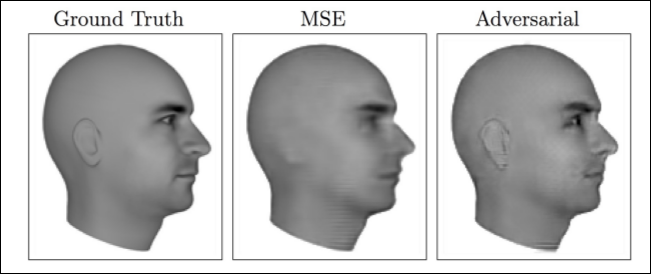
\includegraphics[width=\linewidth,height=0.95\textheight,keepaspectratio]{prezentacja/klatka.png}
\endminipage
\end{frame}

\begin{frame}{Przykład 2 - wysoka rozdzielczość}
\minipage{\textwidth}
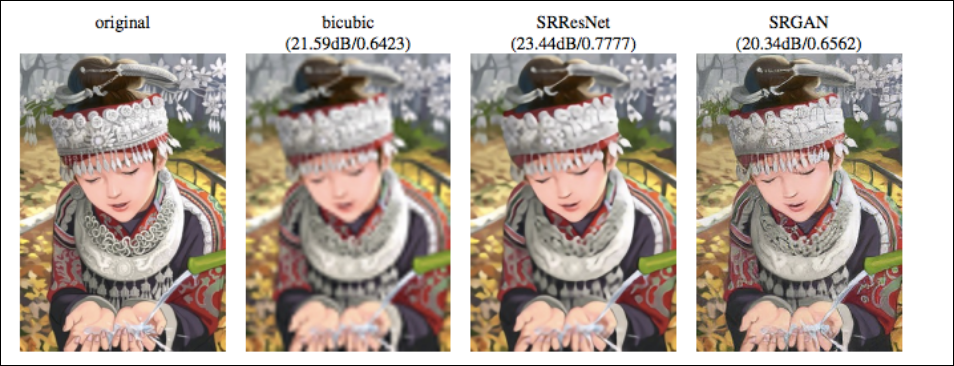
\includegraphics[width=\linewidth,height=0.95\textheight,keepaspectratio]{prezentacja/rozdzielczosc.png}
\endminipage
\end{frame}

\begin{frame}{Dyskryminator i generator}
\minipage{\textwidth}
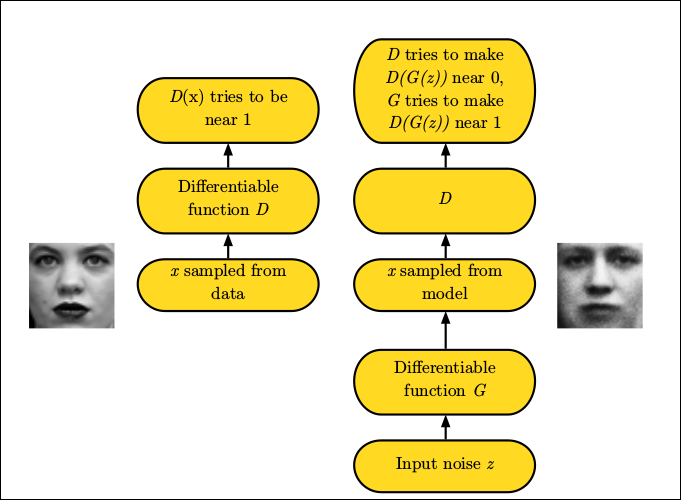
\includegraphics[width=\linewidth,height=0.95\textheight,keepaspectratio]{prezentacja/dyskryminator.png}
\endminipage
\end{frame}

\begin{frame}{Kara, minimax i pierwsze ulepszenia}
\begin{align*}
J^{(D)}(\theta^{(D)}, \theta^{(G)}) &= -\frac{1}{2} \mathbf{E}_{x \sim p_{data}} \log D(x) -\frac{1}{2} \mathbf{E}_{z} \log (1-D(G(z)) \\
J^{(G)} &= -J^{(D)} \\ 
J^{(G)} &=  -\frac{1}{2}\mathbf{E}_{z} \log D(G(z))
\end{align*}
\begin{itemize}
    \item Ostatnie równanie to próba pozbycia się problemu znikającego gradientu kiedy dyskryminator jest zbyt dobry
    \item Równe minibatche
    \item Kroki gradientowe wykonujemy na zmianę
\end{itemize}
\end{frame}

\begin{frame}{Problem 1 - liczba oczu}
\minipage{\textwidth}
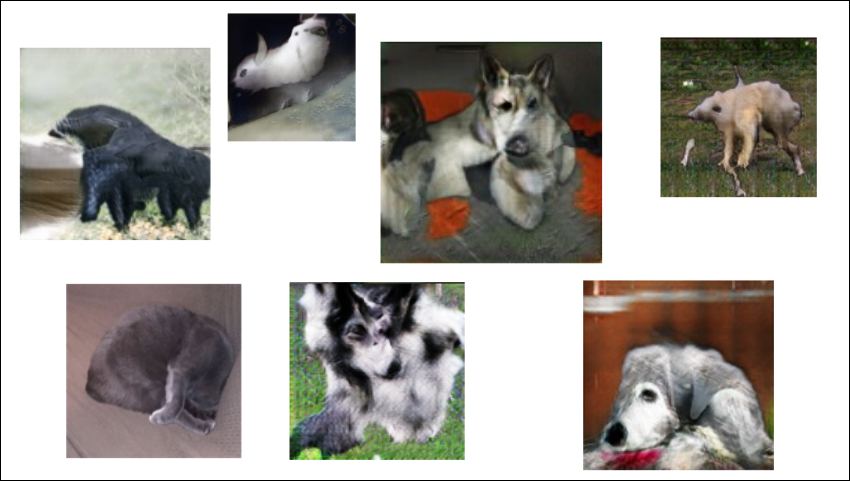
\includegraphics[width=\linewidth,height=0.95\textheight,keepaspectratio]{prezentacja/liczba_oczu.png}
\endminipage
\end{frame}

\begin{frame}{Problem 2 - struktura globalna}
\minipage{\textwidth}
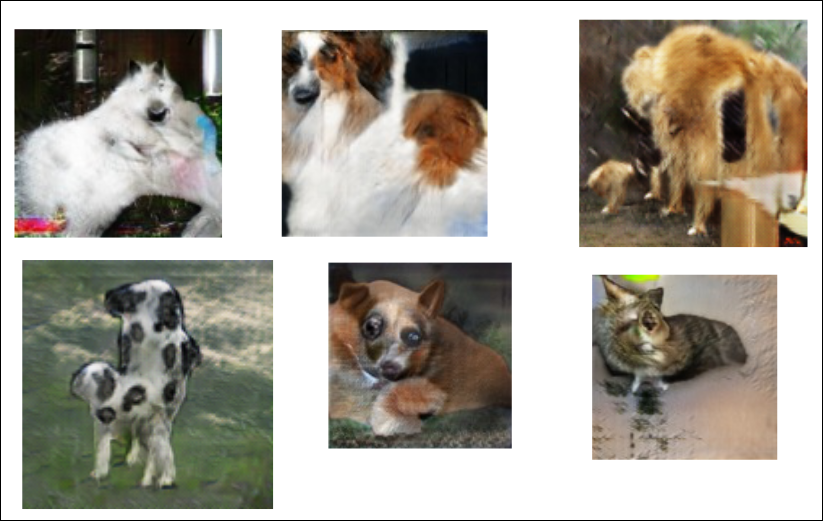
\includegraphics[width=\linewidth,height=0.95\textheight,keepaspectratio]{prezentacja/struktura.png}
\endminipage
\end{frame}


\begin{frame}{Problem 3 - przeskakiwanie między modami}
\minipage{\textwidth}
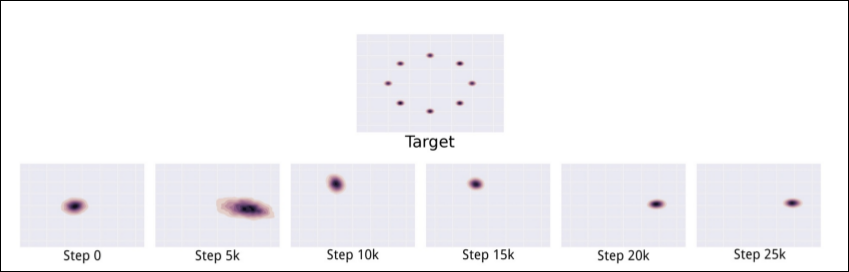
\includegraphics[width=\linewidth,height=0.95\textheight,keepaspectratio]{prezentacja/mody.png}
\endminipage
\end{frame}
    

\begin{frame}{Pozostałe problemy}
\begin{itemize}
    \item Zbyt konkretne odpowiedzi generatora
    \item Generowanie obrazów w wysokiej rozdzielczości
    \item Mała różnorodność wyjść z generatora (problem z modami)
    \item GAN są wrażliwe na duże sygnały (przy ReLU)
\end{itemize}
\end{frame}

\begin{frame}{Co potrafią ulepszone GANy?}
\begin{itemize}
    \item Generowanie twarzy celebrytów w wysokiej rozdzielczości
    \item Realistyczne zdjęcia z CIFAR10, LSUN
    \item Przyspieszenie treningu
\end{itemize}
\end{frame}

\begin{frame}{Stopniowy wzrost}
\minipage{\textwidth}
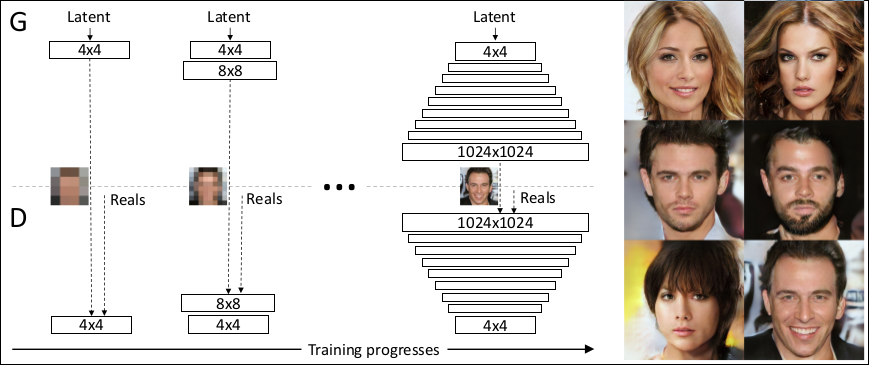
\includegraphics[width=\linewidth,height=0.95\textheight,keepaspectratio]{prezentacja/progressive.png}
\endminipage
\end{frame}

\begin{frame}{Gładkie wprowadzenie warstwy}
\minipage{\textwidth}
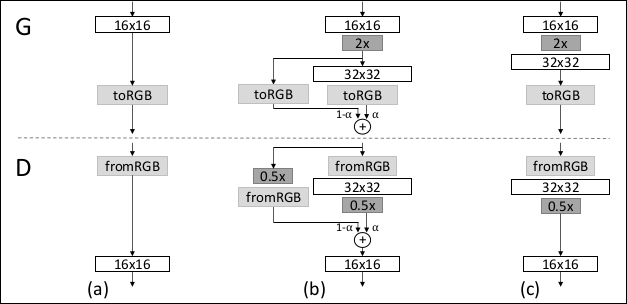
\includegraphics[width=\linewidth,height=0.95\textheight,keepaspectratio]{prezentacja/smooth.png}
\endminipage
\end{frame}

\begin{frame}{Zwiększenie różnorodności}
\begin{itemize}
    \item Idea: feature mapy ze statystykami z całego minibatcha 
    \item Uzasadnienie: odróżnianie modów
    \item Poprzednie prace: dodatkowa warstwa z nauczalnymi wagami do obliczania statystyk
    \item Tutaj: liczymy odchylenie standardowe z każdej cechy (piksela) w każdej lokalizacji i bierzemy średnią ze wszystkich do $S$, a nowa feature mapa to macierz wypełniona $S$
\end{itemize}
\end{frame}

\begin{frame}{Normalizacja}
\begin{itemize}
    \item Ochrona przed zbyt dużym sygnałem (ReLU) - standardowo batch normalization i odpowiednia incjalizacja
    \item Wyrównany learning rate - zamiast inicjalizować uważnie wagi, losujemy z $N(0,1)$. Następnie, zawsze gdy używamy danej wagi skalujemy ją $\hat{w_i} = \frac{w_i}{c}$
    \item $c$ różne dla każdej warstwy
    \item Efekt: Odpowiednio przeskalowany update, lepsza szybkość uczenia
    \item Normalizacja cech per piksel w generatorze
    \item Wzór $$ b_{x,y} = a_{x,y} / \sqrt{\frac{1}{N} \sum_{j=1}^{N} (a_{x,y}^j)^2 + \epsilon}$$
\end{itemize}
\end{frame}

\begin{frame}{Ocenianie skuteczności generatora  - MS-SSIM}
\begin{itemize}
    \item Multi-Scale Structural Similarity (MS-SSIM)
    \item Porównywanie statystyk między obrazkami
    \item Dobrze radzi sobie z wykrywaniem braku modów
    \item Słabo z wykrywaniem różnorodności tekstur i kolorów
\end{itemize}
\end{frame}

\begin{frame}{Ocenianie skuteczności generatora - SWD}
\begin{itemize}
    \item Dystans Wassersteina - jak duży jest koszt przeniesienia jednej chmury punktów na drugą
    $$ W(X,Y)^2 = \min_{\sigma} \sum_{i=1}^N ||X_i - Y_{\sigma(i)} ||^2$$
    \item Sliced Wasserstein Distance (SWD)  - w celu zredukowania kosztów obliczeń, aproksymujemy dystans Wassersteina rzutami na wektory długości $1$ ( w jednowymiarowym przypadku jest wzór na najlepszą permutację) i bierzemy średnią 
    $$ \hat{W(X,Y)} = \int_{\theta \in \Theta} \min_{\sigma} \sum_{i=1}^N  |<X_i-Y_{\sigma(i)}, \theta>|^2 d\theta$$
\end{itemize}
\end{frame}

\begin{frame}{Ocenianie skuteczności generatora - piramida Laplace'a}
\begin{itemize}
    \item Piramida Laplace'a - poziomy rozdzielczości zdjęcia (od $16\times16$ do $128\times128$)
    \item Przebig oceny 
    \begin{enumerate}
        \item Losujemy 16384 obrazków i dla każdego z nich i każdego poziomu piramidy bierzemy 128 jego deskryptorów (wycinki wielkości $7\times7\times3$)
        \item Normalizujemy deskryptory przez średnią i odchylenie standardowe na każdym kolorze
        \item Obliczamy $SWD(\{x_i\},\{y_i\})$
    \end{enumerate}
\end{itemize}
\end{frame}

\begin{frame}{Użyte kary}
\begin{itemize}
    \item Przyczyna: zredukowanie szansy na znikanie gradientu
    \item Least Squares GAN - logarytm w karze zastępujemy kwadratem
    \item Wasserstein GAN - Gradient Penalty - szukanie dyskryminatora odpowiedniej postaci, a dodatkowa kara do WGAN, żeby tą postać wymusić
\end{itemize}
\end{frame}

\begin{frame}{Twarze celebrytów}
\begin{itemize}
    \item CelebA - nieustandaryzowany zbiór obrazów celebrytów (wiele osób, rożne profile, szumy)
\end{itemize}
\minipage{\textwidth}
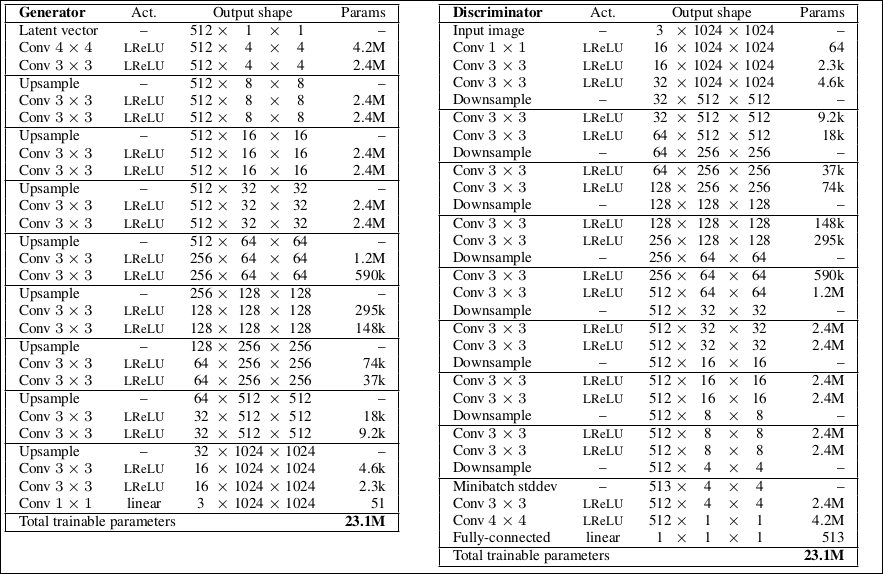
\includegraphics[width=\linewidth,height=0.65\textheight,keepaspectratio]{prezentacja/architektura.png}
\endminipage
\end{frame}

\begin{frame}{Wyniki na CelebA}
\minipage{\textwidth}
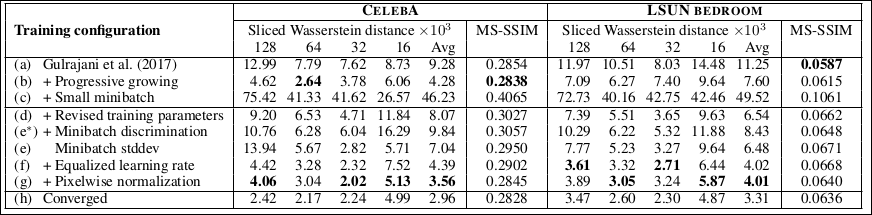
\includegraphics[width=\linewidth,height=0.95\textheight,keepaspectratio]{prezentacja/scores.png}
\endminipage
\end{frame}

\begin{frame}{Czas treningu}
\minipage{\textwidth}
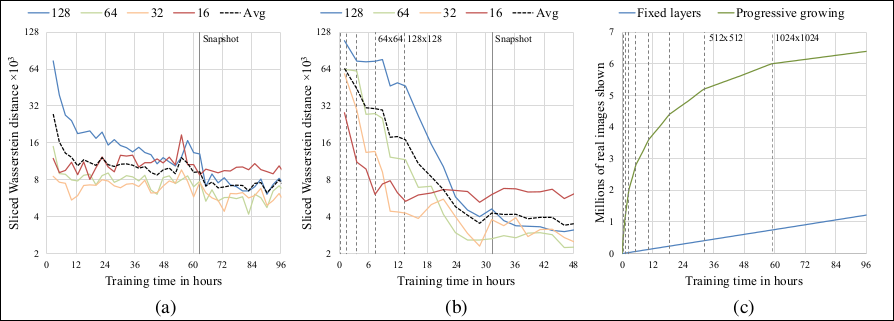
\includegraphics[width=\linewidth,height=0.95\textheight,keepaspectratio]{prezentacja/czas_treningu.png}
\endminipage
\end{frame}

\begin{frame}{Twarze celebrytów - CelebA-HQ}
\minipage{\textwidth}
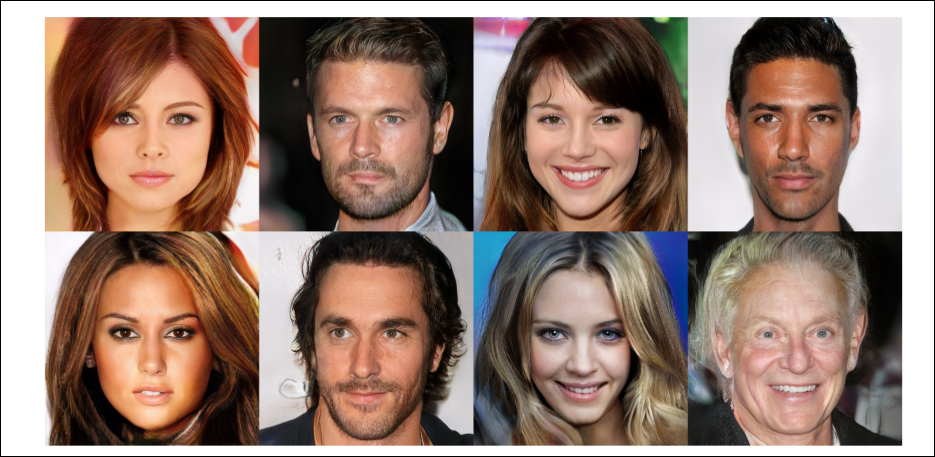
\includegraphics[width=\linewidth,height=0.95\textheight,keepaspectratio]{prezentacja/twarze1.png}
\endminipage
\end{frame}

\begin{frame}{Pozostałe przykłady}
\begin{itemize}
    \item Zdjęcia z Appendixu H
    \item \href{https://www.youtube.com/watch?v=G06dEcZ-QTg}{Film - prezentacja wyników}
\end{itemize}    
\end{frame}
    
\begin{frame}{Bibliografia} 

\nocite{*}
\bibliography{biblio1}
\bibliographystyle{plain}
\end{frame}

\appendix
\backupbegin

\backupend
\end{document}
